\documentclass[spanish]{article}
\usepackage{titlesec}

\renewcommand{\contentsname}{Plan de la charla}

%Paquetes
\usepackage[left=4cm, right=4cm]{geometry}
\usepackage{palatino}%Fuente
\usepackage{graphicx}%Imágenes
\usepackage{float}%Imágenes
\usepackage{subcaption}%Imágenes
\usepackage{enumitem}%Listas
\usepackage{parskip}%Espacio entre párrafos
\usepackage{multicol}
\usepackage{amsthm}%Mate
\usepackage{amssymb}%Mate
\usepackage{amsmath}%Mate
\usepackage{tikz}%Mate (diagramas)
\usepackage{dutchcal}
\usepackage{tikz-cd}
\usepackage{xcolor}

\usetikzlibrary{%
	matrix,%
	calc,%
	arrows,%
	shapes,
	decorations.markings
}
\usepackage[bookmarks,bookmarksopen,bookmarksdepth=3]{hyperref}%Links a lugares en el texto
\hypersetup{%colores
	colorlinks=true,
	urlcolor=blue,
	linkcolor=magenta,
	citecolor=blue,
	filecolor=blue,
	urlbordercolor=white,
	linkbordercolor=white,
	citebordercolor=white,
	filebordercolor=white
}
\usepackage{cleveref}
\crefname{section}{sección}{secciones}


%Referencias
\usepackage[style=authortitle,backend=bibtex]{biblatex}
\addbibresource{de-rham-bib.bib}

\theoremstyle{definition}
\renewcommand{\proofname}{Demostración}

\newtheorem*{defn}{Definición}
\newtheorem*{teo}{Teorema}
\newtheorem*{prop}{Proposición}
\newtheorem*{coro}{Corolario}
\newtheorem*{lema}{Lema}
\newtheorem*{obs}{Observación}
\newtheorem{ejer}{Ejercicio}
\newtheorem*{ejer*}{Ejercicio}
\newtheorem*{af}{Afirmación}
\newtheorem*{ejem}{Ejemplo}
\newtheorem*{pregunta}{Pregunta}

\newcommand{\R}{\mathbb{R}}
\newcommand{\Z}{\mathbb{Z}}
\newcommand{\N}{\mathbb{N}}
\newcommand{\C}{\mathbb{C}}
\newcommand{\Q}{\mathbb{Q}}
\newcommand{\D}{\mathbb{D}}
\newcommand{\Hy}{\mathbb{H}}
\newcommand{\X}{\mathfrak{X}}
\newcommand{\T}{\mathfrak{T}}
\newcommand{\Cinf}{C^\infty}

\DeclareMathOperator{\End}{End}
\DeclareMathOperator{\sen}{sen}
\DeclareMathOperator{\img}{img}
\DeclareMathOperator{\Arg}{Arg}
\DeclareMathOperator{\Id}{Id}
\DeclareMathOperator{\Alt}{Alt}
\DeclareMathOperator{\sgn}{sgn}
\DeclareMathOperator{\supp}{supp}
\DeclareMathOperator{\Hom}{Hom}


\begin{document}
	\begin{center}
		{\LARGE Cohomología de de Rham}
		
		\href{https://github.com/dan-gc/de-rham/blob/main/de-rham.pdf}{github.com/dan-gc/de-rham}
	\end{center}
	\tableofcontents
	\vspace{.5cm}
	\textit{Nota bibliográfica.} La \cref{sec:1} es la introducción de \cite{Bott}. Las \cref{sec:2,sec:3,sec:4} son una mezcla de \cite{Lee} y \cite{Loring}, y un poco de \cite{Bott}. La sección \cref{sec:5} está en \cite{Lee}.

	\section{Motivación}\label{sec:1}
	Las componentes conexas de un espacio $X$ están caracterizadas por el hecho de que, en cada una, \textit{cualquier función localmente constante es globalmente constante}. Definendo $H^0(X)$ como el espacio vectorial de funciones real-valuadas localmente constantes, $\dim H^0(X)$ es el número de componentes conexas de $X$.
	
	Ahora observemos que si $M$ es un abierto en $\R^n$, esta propiedad se describe pidiendo que el gradiente
	\[df=\sum_i\frac{\partial f}{\partial x^i}dx^i\]
	sea cero. Buscamos una ecuación diferencial natural que nos ayude a definir $H^1(X)$.
	
	Ahora para generalizar esta idea tomemos una 1-forma $\theta=\sum_ia_idx^i$ y la pensamos como un operador sobre las curvas en $M$ vía
	\[\gamma\mapsto\int_\gamma\theta\]
	Y se nos antoja que $\theta$ sea \textit{localmente} constante en el sentido de que al variar ligeramente $\gamma$ (sin cambiar los puntos inicial y final) la intergral permanece igual. ¿A qué nos referimos con esto?
	
	\[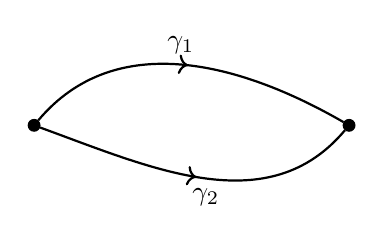
\begin{tikzpicture}
		[decoration={markings,mark=at position 0.5 with {\arrow{>}}},
		witharrow/.style={postaction={decorate}},
		dot/.style={draw,fill,circle,inner sep=1.5pt,minimum width=0pt}
		]
		
		% ellipse
		\begin{scope}[shift={(5,0)}]
			\node[dot] (a3) at (0,0) {};
			\node[dot] (b3) at (4,0) {};
			\draw[thick,witharrow] (a3) to[out=50,in=150]node[above]{$\gamma_1$} (b3);
			
			%\foreach \o/\i in {40/160,30/170,20/180,10/190,-10/200}
			%\draw (a3) to[out=\o,in=\i]  (b3);
			
			\draw[thick,witharrow] (a3) to[out=-20,in=-130]node[below]{$\gamma_2$} (b3);
			
			\node at ($(a3)+(0.5,0.8)$) (X3) {};
		\end{scope}
	\end{tikzpicture}\]
	
	Si las integrales sobre dos curvas homotópicas $\gamma_1$ y $\gamma_2$ coinciden,
	\[\int_{\gamma_1}\theta=\int_{\gamma_2}\theta\]
	es decir
	\[0=\int_{\gamma_1}\theta-\int_{\gamma_2}\theta=\int_{\gamma_1-\gamma_2}\theta=\int_{\partial D^2}\theta=\int_{D^2}d\theta,\]
	así que si $d\theta=0$ la 1-forma es \textit{localmente constante} en el espacio de lazos.
	
	Ahora notemos que por el teorema fundamental del cálculo $\int_\gamma df=f(Q)-f(P)$ donde $P$ y $Q$ son los puntos inicial y final de $\gamma$. Diremos que los gradientes (0-formas exactas) son \textbf{\textit{trivialmente}} localmente constantes.
	
	Definamos entonces $H^1(M)$ como el espacio vectorial de integrales de línea localmente constantes módulo las que son trivialmente constantes.
	
	\section{Complejo de de Rham}\label{sec:2}
	En esta sección construimos un funtor contravariante $\Omega^*(-)$ de la categoría de variedades suaves en la categoría de álgebras diferenciales graduadas asociativas y anticonmutativas. A cada álgebra corresponde un complejo de cadenas que llamaremos complejo de de Rham.
	\begin{enumerate}
		\item Una variedad topológica $M$ es \textbf{\textit{diferenciable}} si tiene un atlas tal que las funciones de transición son difeomorfismos. 
		%\linebreak${\psi\circ\varphi^{-1}:\R^n\to\R^n}$ son $\Cinf$-diferenciables. 
		El atlas debe ser maximal en el sentido de que contiene todas las posibles cartas que son compatibles.
		
		Si $u^1,\ldots,u^n$ son las funciones coordenadas de $\R^n$ y $(U,\varphi)$ es una carta coordenada de $M$, podemos escribir $\varphi=(x^1,\ldots,x^n)$ donde  $x^i=u^i\circ\varphi$. Una función real-valuada $f$ definida en $M$ es \textbf{\textit{suave}} si su \textbf{\textit{pullback}} $f\circ\varphi^{-1}$ es $\Cinf$-diferenciable. La colección de tales funciones se denota por $\Cinf(M)$.
		
		\item En cada punto $p\in M$ con carta coordenada $(U,x^1,\ldots,x^n)$ el conjunto de funcionales $\Cinf(M)\to \R$
		\[\frac{\partial}{\partial x^1}\Big|_p,\ldots,\frac{\partial}{\partial x^n}\Big|_p\]
		definidos mediante $f\mapsto \frac{\partial f\circ\varphi^{-1}}{\partial u^i}\Big|_p$ generan un espacio vectorial que llamamos \textbf{\textit{espacio tangente}} y denotamos por $T_pM$. Un \textbf{\textit{campo vectorial}} es una sección suave del \textbf{\textit{haz tangente}} $TM=\bigcup_{p\in M}T_pM$.
		
		El conjunto de funcionales $T_pM\to \R$
		\[(dx^1)_p,\ldots,(dx^n)_p\]
		definidos mediante $(dx^i)_p\left(\frac{\partial}{\partial x^j}\Big|_p\right)=\delta_j^i$ generan un espacio vectorial que llamamos \textbf{\textit{espacio cotangente}} y denotamos por $T_p^*M\approx\Hom(T_pM,\R)$. Sus elementos se llaman \textbf{\textit{1-covectores}}.
		
		\item Nuestro siguiente paso es construir el funtor $\bigwedge^k(-)$ que a un espacio vectorial arbitrario asigna el espacio vectorial de \textbf{\textit{$k$-tensores alternantes}}. Aplicaremos este funtor al espacio tangente en un punto, luego variamos el punto para obtener secciones de un haz y finalmente tomamos la suma directa sobre $k$. El resultado es un álgebra graduada asociativa y anticonmutativa a la que después dotaremos de una antiderivación.
		
		Las funciones $\R$-multilineales lineales $\underbrace{T_pM\times\ldots\times T_pM}_{k\text{ veces}}\to \R$ se llaman \textbf{\textit{$k$-tensores}}. Un $k$-tensor es un \textbf{\textit{$k$-covector}} si es \textbf{\textit{alternante}}
		%en el sentido de que $f(v_{\sigma(1)},\ldots,v_{\sigma(k)})=(\sgn\sigma)f(v_1,\ldots,v_k)$ para cualesquiera $v_1,\ldots,v_k\in T_pM$. Equivalentemente,
		, es decir, si su valor cambia de signo cuando dos entradas cambian de lugar. La colección de $k$-covectores en $p$ se denota por $\bigwedge^k(T^*_pM)$.
		
		Una \textbf{\textit{$k$-forma}} o \textbf{\textit{campo $k$-covectorial}} es una
		% función que a cada punto de $M$ le asocia un $k$-covector. Es una 
		sección suave del haz vectorial $\bigwedge^k(T^*M)=\bigcup_{p\in M}\bigwedge^k(T_p^*M)$.  La colección de $k$-formas en $M$ se denota por $\Omega^k(M)$.
		
		
		\item El \textbf{\textit{producto cuña}} definido puntualmente como el $(k+\ell)$-covector
		\[(\omega\wedge\tau)_p=\frac{1}{k!\ell!}\operatorname{Alt}(\omega\otimes\tau)_p\]
		%donde $\operatorname{Alt}(\omega_p)(v_1,\ldots,v_k)=\sum_{\sigma\in S_k}\omega_p(v_{\sigma(1)},\ldots,v_{\sigma(k)})$.
		que explícitamente quiere decir que
		\[(\omega\wedge\tau)_p(v_1,\ldots,v_{k+\ell})=\sum_{\sigma\in S_{k+\ell}}(\sgn\sigma)\omega_p(v_{\sigma(1)},\ldots,v_{\sigma(k)})\tau_p(v_{\sigma(k+1)},\ldots,v_{\sigma(k+\ell)})\]
		para $\omega\in\Omega^k(M)$ y $\tau\in\Omega^\ell(M)$, donde $S_{k+\ell}$ es el grupo de permutaciones. Esta operación se extiende suavemente a una $(k+\ell)$-forma.
		
		\textcolor{blue}{Recordemos que el \textbf{\textit{producto copa}} entre las cocadenas $\varphi\in C^k(X;R)$ y $\psi\in C^\ell(X;R)$ está definido como
			\[(\varphi\smile \psi)(\sigma)=\varphi(\sigma|[v_0,\ldots,v_k])\psi(\sigma|[v_{k+1},\ldots,v_{\ell}])\]
			para un simplejo singular $\sigma:\Delta_{k+\ell}\to X$. (El símbolo $[v_0,\ldots,v_k]$ representa el simplejo dado por los vértices $v_0,\ldots,v_k$).
		}
		
		El producto cuña es bilineal, asociativo y anticonmutativo:
		\[\omega\wedge\tau=(-1)^{\deg\omega\deg\tau}\tau\wedge\omega\]
		
		Una base de $\bigwedge^k(T_p^*U)$ en una vecindad coordenada $U$ está dada por los $k$-covectores
		\[dx^{i_1}\wedge\ldots\wedge dx^{i_k}\qquad \text{con }i_1<\ldots<i_k\]
		así que es un espacio vectorial de dimensión $\binom{n}{k}$.
		\iffalse
		Conviene pensar en estos objetos , para los 1-covectores $\omega^1,\ldots,\omega^k$ y los vectores $v_1,\ldots,v_k$,
		\[\omega^1\wedge\ldots\wedge\omega^k(v_1,\ldots,v_k)=\det(\omega^i(v_j))\]
		Por ejemplo, en $\R^2$, $dx\wedge dy\left(\begin{pmatrix}
			v^1\\
			v^2
		\end{pmatrix},\begin{pmatrix}
			w^1\\
			w^2
		\end{pmatrix}\right)=v^1w^2-v^2w^1$.\fi
		
		El conjunto $\Omega^*(M)=\bigoplus_k^n\Omega^k(M)$ es un álgebra graduada asociativa y anticonmutativa con el producto cuña como operación.
		%Cada elemento de $\Omega^*(M)$ se puede escribir de manera única como una suma $\sum_{k=0}^n\omega_k$ con $\omega_k\in\Omega^k(M)$.
		
		
		\item La \textbf{\textit{derivada exterior de una función real-valuada}} $f\in\Cinf(M)=\Omega^0(M)$ es la 1-forma definida localmente como
		\[df=\sum\frac{\partial f}{\partial x^i}dx^i\]
		o, equivalentemente, es el operador que manda $v\mapsto vf$ para $v\in T_pM$. (Esta definición local se extiende a una 1-forma).
		
		La \textbf{\textit{derivada exterior}} es el operador $d:\Omega^*(M)\to\Omega^*(M)$ definido localmente como
		\[d\omega=d\sum_Ia_Ix^I =\sum_Ida_I\wedge x^I=\sum_I\sum_j\frac{\partial a_I}{\partial x^j}dx^j\wedge x^I,\]
		(se extiende correctamente) que satisface las siguientes propiedades:
		\begin{enumerate}
			\item Es $\R$-lineal.
			\item $d(\omega\wedge\tau)=(d\omega)\wedge\tau+(-1)^{\deg\omega}\omega\wedge(d\tau)$
			\item $d^2=0$
			\item Si $f\in\Cinf(U)$ y $X$ es un campo vectorial, entonces $(df)(X)=Xf$.
			
		\end{enumerate}
		\textcolor{blue}{El \textbf{\textit{operador frontera en cohomología singular}} es simplemente $\Hom(\partial)=\partial^*$ donde $\partial$ es la frontera de cadenas singulares. Recordando la definición del mapeo inducido mediante el funtor contravariante $\Hom$, tenemos:}
		\[\begin{tikzcd}
			\textcolor{blue}{C_{n+1}}\arrow[d,blue,swap,"\partial"]\arrow[rd,blue,"\varphi\circ\partial=\partial^*"]\\	\textcolor{blue}{C_n}\arrow[blue,swap,r,"\varphi"]&\textcolor{blue}{G}
		\end{tikzcd}\]
		\textcolor{blue}{que no es más que evaluar el cociclo $\varphi$ en la frontera de una cadena (simplejo), es decir, en la suma alternada de las caras del simplejo:}
		\[\color{blue}\varphi\partial (\sigma)=\sum_i(-1)^i\varphi(\sigma|[v_1,\ldots,\hat{v}_i,\ldots,v_{n+1}])\]
		
		Una $k$-forma $\omega$ es \textbf{\textit{cerrada}} si $d\omega=0$ y \textbf{\textit{exacta}} si existe $\eta\in\Omega^{k-1}(M)$ tal que $d\eta=\omega$.
		
		
		\item Dada una función suave $F:N\to M$ entre variedades y un $k$-covector $\omega_{F(p)}\in T^*_{F(p)}M$, el \textbf{\textit{pullback}} de $\omega_{F(p)}$ es el $k$-covector en $T_p^*N$ dado por
		\[(F^*\omega)_p(v_1,\ldots,v_k)=\omega_{F(p)}(F_{*,p}v_1,\ldots,F_{*,p}v_k)\]
		para $v_1,\ldots,v_k\in T_pN$ donde $F_{*,p}$ es la diferencial de $F$ definida por $F_{*,p}vf=v(f\circ F)$.
		
		
		\begin{prop}[Propiedades del pullback]
			Si $F:M\to N$ es una función suave entre variedades y $\omega$ y $\tau$ son formas diferenciales en $M$,
			\begin{enumerate}
				\item $F^*:\Omega^k(N)\to\Omega^k(M)$ es $\R$-lineal.
				\item $F^*(\omega\wedge\tau)=F^*\omega\wedge F^*\tau$.
				\item En cualquier carta coordenada,
				\[F^*\left(\sum\omega_Idy^{i_1}\wedge\ldots\wedge dy^{i_k}\right)=\sum(\omega_I\circ F)d(y^{i_1}\circ F)\wedge\ldots\wedge d(y^{i_k}\circ F)\]
				donde $d$ denota la diferencial.
			\end{enumerate}
		\end{prop}
		
		\begin{prop}[Naturalidad de la derivada exterior]
			Si $F:N\to M$ es una función suave entre variedades y $\omega\in\Omega^k(M)$, entonces
			\[dF^*\omega=F^*d\omega\]
		\end{prop}
		
		
		
		
	\end{enumerate}
	\iffalse
	\begin{obs}[Tres formas de ver la derivada de una función real-valuada]
		Sea $f\in\Cinf(M)$. Los siguientes tres objetos están en correspondencia:
		\begin{enumerate}
			\item La diferencial $f_{*,p}:T_pM\to T_{f(p)}\R$ que manda $v$ al vector $f_{*,p}v$ dado por $\Cinf(\R)\ni g\mapsto v(g\circ f)$.
			\item La 1-forma $df\in \Omega^1(M)$ obtenida mediante la derivada exterior de $f$, definida por $df(v)=vf$, evaluada en $p$.
			\item La función que a una curva $\gamma:(-\varepsilon,\varepsilon)\to M$ con $\gamma(0)=p$ y $\gamma'(0)=v$ le asocia el número real $(f\circ \gamma)'(0)$.
		\end{enumerate}
	\end{obs}
	\fi
	
	\section{Cohomología de de Rham}\label{sec:3}
	Ahora construimos el funtor $H_{dR}^p(-)$.
	\begin{enumerate}
		\item La \textbf{\textit{$k$-ésima cohomología de de Rham}} es el espacio vectorial cociente
		\[H_{dR}^k=\frac{\{k\text{-formas cerradas}\}}{\{k\text{-formas exactas}\}}\]
		
		\item (Funtorialidad) Sea$F:M\to N$ es una función suave. Como el pullback $F^*:\Omega^k(N)\to\Omega^k(M)$ conmuta con la derivada exterior, manda formas cerradas en cerradas y exactas en exactas, así que desciende a homología y tenemos un \textbf{\textit{pullback en homología}}, que también denotamos por $F^*$, tal que
		\begin{enumerate}
			\item Si $G:N\to P$ es otra función suave, $(G\circ F)^*=G^*\circ F^*$
			\item $\Id^*$ es la identidad en $H_{dR}^k(M)$.
		\end{enumerate}
		es decir, $H_{dR}^k(-)$ es un funtor contravariante de variedades (con frontera) en espacios vectoriales.
		
		\item (Invarianza homotópica) Si $M$ y $N$ son homotópicamente equivalentes, $H_{dR}^k(M)\approx H_{dR}^k(N)$ para toda $k$. El isomorfismo es el inducido por cualquier equivalencia homotópica, ya que dos funciones equivalentemente homotópicas inducen el mismo mapeo en cohomología.
		
		(Lema de Poincaré) Si $M$ es contraible, $H_{dR}^p(M)\approx0$ para $p\geq1$.
		
		\item Resultados básicos:
		\begin{enumerate}
			\item (Cohomología de la unión disjunta) Si $M=\bigsqcup M_i$, entonces $H_{dR}^p(M)\approx \prod H_{dR}^p(M_i)$. Usando el pullback de las inclusiones.
			
			\item (Cohomología de grado cero) $H_{dR}^0(M)\approx\R$ por ser el espacio de funciones constantes, es decir, soluciones de $df=0$.
			
			\item (Mayer-Vietoris) Supongamos que $\{U,V\}$ es una cubierta abierta de $M$. Las inclusiones
			\[\begin{tikzcd}[column sep=small,row sep=small]
				&U\arrow[dr,"k"]\\
				U\cap V\arrow[ru,"i"]\arrow[dr,swap,"j"]&&M\\
				&V\arrow[ru,swap,"l"]
			\end{tikzcd}\]
			inducen la siguiente sucesión exacta larga en cohomología:
			\[\begin{tikzcd}[column sep=small]
				\cdots\arrow[r,"\delta"]&H_{dR}^p\arrow[r,"k^*\oplus l^*"]&H_{dR}^p(U)\oplus H_{dR}^p(V)\arrow[r,"i^*-j^*"]&H_{dR}^p(U\cap V)\arrow[r,"\delta"]&H_{dR}^{p+1}(M)\arrow[r,"k^*\oplus l^*"]&\cdots
			\end{tikzcd}\]
		\end{enumerate}
		
		\item El \textbf{\textit{soporte}} de una forma $\omega$ en $M$ es $\supp \omega=\overline{\{p\in M:\omega(p)\neq0\}}$. La colección de $p$-formas con soporte compacto en $M$ se denota por $\Omega_c^p(M)$. La \textbf{\textit{$p$-ésima cohomología con soporte compacto de $M$}} es el espacio vectorial cociente
		\[H^p_c(M)=\frac{\ker d:\Omega_c^p(M)\to \Omega_c^{p+1}(M)}{\img d:\Omega_c^{p-1}\to\Omega_c^p(M})\]
	\end{enumerate}
	\begin{ejem}[La cohomología compacta de $\R$]
		Como no hay funciones constantes no cero con soporte compacto, $H^0(\R)\approx 0$. Consideremos el mapeo
		\[\int_\R:\Omega_c^1(\R)\to\R\]
		Es suprayectivo por la existencia de funciones flan. Veamos que su kernel son las 1-formas exactas con soporte compacto. Por un lado, si $df$ tiene soporte contenido en un intervalo $[a,b]$,
		\[\int_\R df=\int_a^bdf=f(b)-f(a)=0-0.\]
		Por otro lado, si $g(x)dx$ tiene integral cero en $\R$, su antiderivada
		\[f(x)=\int_{-\infty}^xg(t)dt\]
		tiene soporte compacto.			
	\end{ejem}
	\iffalse
	\begin{ejem}
		En general,
		\[H^p_c(\R^n)\approx\begin{cases}
			\begin{aligned}
				0\qquad&\text{si }p< n\\
				\R\qquad&\text{si }p=n
			\end{aligned}
		\end{cases}\]
	\end{ejem}
	\fi
	
	\section{Integración en variedades}\label{sec:4}
	\begin{defn}[Orientación]\leavevmode
		
		Dos bases de $T_pM$ están \textbf{\textit{consistentemente orientadas}} si la matriz de cambio de base tiene determinante positivo. Una \textbf{\textit{orientación puntual}} en $M$ es una elección de clase de equivalencia de bases en cada espacio tangente. 
		
		Un \textbf{\textit{marco local}} (una $n$-tupla de secciones del haz tangente $TU$ en un abierto $U$ que en cada punto son una base de $T_pU$) está \textbf{\textit{positivamente orientado}} si en cada punto es una base en la orientación de $M$. Si cada punto está en el dominio de un marco local orientado, $M$ es \textbf{\textit{orientable}}.
		
		$M$ es orientable si y sólo si existe una $n$-forma que no se anula y es positiva en cualquier marco local orientado que llamamos \textbf{\textit{forma de orientación}}. Si $M$ es Riemanniana orientada existe una única \textbf{\textit{forma de volumen}} $dV$ que vale 1 en cualquier marco local ortonormal orientado de $TM$ y, equivalentemente, en cualesquiera coordenadas locales orientadas $x^1,\ldots,x^n$ se expresa como
		\[dV_g=\sqrt{\det g_{ij}}dx^1\wedge\ldots\wedge dx^n\]
		donde $g_{ij}=\left\langle\frac{\partial}{\partial x^i},\frac{\partial}{\partial x^j}\right\rangle$.
	\end{defn}
	
	%Una variedad es \textit{\textbf{orientable}} si existe una $n$-forma en $M$ que no se anula. (El espacio de $n$-formas en una $n$-variedad es de dimensión 1). Una \textbf{\textit{orientación}} es la elección de una de las dos posibles  clases de equivalencia de $n$-formas en $M$ que no se anulan.
	\iffalse
	\begin{defn}[Integrales de línea]\leavevmode
		\begin{enumerate}
			\item Primero definimos la integral de una 1-forma $\omega$ en un intervalo $[a,b]\subset\R$. Para la coordenada natural $t$ en $\R$, sabemos que $\omega_t=f(t)dt$ para alguna función suave $f:[a,b]\to\R$. Definimos \textbf{\textit{la integral de $\omega$ en $[a,b]$}} como la integral de Riemann:
			\[\int_{[a,b]}\omega=\int_a^bf(t)dt\]
			
			\item La generalización a una curva sobre una variedad está dada por el pullback de la forma bajo la carta coordenada. Si $\gamma:[a,b]\to M$ es una curva suave y $\omega$ es un campo covectorial suave en $M$, la \textbf{\textit{integral de $\omega$ sobre $\gamma$}} es el número real
			\[\int_\gamma\omega=\int_{[a,b]}\gamma^*\omega\]
		\end{enumerate}
	\end{defn}
	
	\begin{prop}[Propiedades de las integrales de línea]
		Sea $M$ una variedad suave, $\gamma:[a,b]\to M$ una curva suave y $\omega$ una 1-forma en $M$. Entonces
		\begin{enumerate}
			\item La integral de $\omega$ en $\gamma$ es $\R$-lineal en $\X^*(M)$, es decir, si $a,b\in\R$ y $\omega_1,\omega_2\in\X^*(M)$,
			$\int_\gamma(a\omega_1+b\omega_2)=a\int_\gamma\omega_1+b\int_\gamma\omega_2$.
			\item Si $\gamma$ es constante, $\int_\gamma\omega=0$.
			\item SI $\gamma_1=\gamma|_{[a,b]}$ y $\gamma_2=\gamma|_{[b,c]}$ con $a<b<c$, entonces
			$\int_\gamma\omega=\int_{\gamma_1}\omega+\int_{\gamma_2}\omega$.
			\item
			Si $F:N\to M$ es una función suave,
			\[\int_\gamma F^*\omega=\int_{F\circ \gamma}\omega\]
			\item Hay otra expresión para esta integral: \[\int_\gamma\omega=\int_a^b\omega_{\gamma(t)}(\gamma'(t))dt\]
		\end{enumerate}
	\end{prop}
	\begin{teo}[Fundamental de las integrales de línea]
		Sea $M$ una variedad suave. Si $f$ es una función suave real-valuada en $M$ y $\gamma:[a,b]\to M$ es una curva suave, entonces
		\[\int_\gamma df=f(\gamma(b))-f(\gamma(a)).\]
	\end{teo}
	\fi
	\begin{obs}[Integración en variedades]\leavevmode
		\begin{itemize}
			\item Sólo podemos integrar variedades orientadas.
			\item Sólo podemos integrar $n$-formas en una variedad de dimensión $n$.
			\item Las $n$-formas que integremos deben tener soporte compacto.
		\end{itemize}
	\end{obs}
	\begin{defn}[Integración en variedades]\leavevmode
		\begin{enumerate}
			\item Primero definimos \textit{\textbf{la integral de una $n$-forma}} en $\R^n$. Si $\omega=f(x)dx^1\wedge\ldots\wedge dx^n$ es una $n$-forma en un abierto $U\subset\R^n$, su integral en $A\subset U$ es la integral de Riemann de $f$:
			\[\int_A\omega=\int_Af(x)dx^1\wedge\ldots\wedge dx^n:=\int_Af(x)dx^1\ldots dx^n\]
			(la integral de Riemann es el supremo de las sumas inferiores y el ínfimo de las sumas superiores sobre particiones de rectángulos).
			
			\item Denotamos por $\Omega_c^k(M)$ el conjunto de $k$-formas en $M$ que tienen soporte compacto. En una variedad orientada $M$ de dimensión $n$ con una carta coordenada orientada $U$ definimos para $\omega\in\Omega_c^n(U)$,
			\[\int_U\omega:=\int_{\varphi(U)}(\varphi^{-1})^*\omega\]
			\item Dada una partición de la unidad $\{\rho_\alpha\}$ subordinada al atlas orientado $\{(U_\alpha,\varphi_\alpha)\}$ de $M$ y $\omega\in\Omega_c^n(M)$, tenemos que
			\begin{itemize}
				\item $\omega=\sum_\alpha\rho_\alpha\omega$ es una suma finita en cada punto.
				\item $\supp \rho_\alpha\omega$ es compacto.
				\item $\rho_\alpha\omega$ es una $n$-forma con soporte compacto en $U_\alpha$, así que su integral $\int_{U_\alpha}\rho_\alpha\omega$ está bien definida.
			\end{itemize}
			Podemos definir
			\[\int_M\omega:=\sum_\alpha\int_{U_\alpha}\rho_\alpha\omega\]
			que es independiente de la elección de atlas orientado y partición de la unidad.
			
			Si $(M,g)$ es Riemanniana orientada y compacta definimos
			\[\operatorname{Vol}(M):=\int_MdV_g\]
		\end{enumerate}
	\end{defn}
	
	\begin{prop}[Propiedades de integración en variedades]
		Sean $M$ y $N$ variedades diferenciables orientadas de dimensión $n$ con o sin frontera y $\omega$ y $\eta$ dos $n$-formas con soporte compacto en $M$.
		\begin{enumerate}
			\item \textbf{Linealidad.} Si $a,b\in\R$, entonces $\int_Ma\omega+b\eta=a\int_M\omega+b\int_M\eta$.
			
			\item \textbf{Revierte orientación.} Si $-M$ denota la orientación contraria de $M$, $-\int_M\omega=\int_{-M}\omega$.
			
			\item \textbf{Positividad.} Si $\omega$ está positivamente orientada, $\int_M\omega>0$.
			
			\item \textbf{Invarianza bajo difeomorfismos.} Si $F:N\to M$ es un difeomorfismo, $\int_M\omega=\int_M F^*\omega$ si $F$ preserva orientación, y si la revierte una es inversa aditiva de la otra.
		\end{enumerate}
	\end{prop}
	\begin{prop}[Integración sobre parametrizaciones]
		Sean $M$ es una $n$-variedad orientada con o sin frontera y $\omega$ una $n$-forma con soporte compacto en $M$. Suponamos que $D_1,\ldots,D_k$ son dominios de integración en $\R^n$, y para $i=1,\ldots,k$, tenemos mapeos suaves $F_i:\bar{D}_i\to M$ tales que:
		\begin{enumerate}
			\item $F_i$ se restringe a un mapeo que preserva orientación de $D_i$ en un abierto $W_i\subset M$,
			\item $W_i\cap W_j\neq\varnothing$ para $i\neq j$,
			\item $\supp \omega\subseteq\bar{W}_1\cup\ldots\cup\bar{W}_k$.
		\end{enumerate}
		Entonces,
		\[\int_M\omega=\sum_{i=1}^k\int_{D_i}F^*_i\omega\]
	\end{prop}
	\begin{prop}[Pullback de formas de grado máximo]
		Si $F:M\to N$ es una función suave entre las variedades $M$ y $N$ con con coordenadas locales $(x^i)$ en $U\subset M$ y $(y^i)$ en $V\subset N$, y si $u$ es cualquier función real-valuada en $N$,
		\[F^*(udy^1\wedge\ldots\wedge dy^n)=(\det DF)(u\circ F)dx^1\wedge\ldots\wedge dx^n\]
		donde $DF$ es la matriz jacobiana de la diferencial $F_*$.
	\end{prop}
	
	\begin{defn}
		Una variedad con frontera $M$ es una $n$-variedad localmente homeomorfa al semiplano superior. Los puntos cuya $n$-ésima coordenada es cero conforman la \textbf{\textit{frontera de $M$}}, que denotamos por $\partial M$. Si $\{(U_\alpha,\varphi_\alpha)\}$ es un atlas en $M$, el atlas $\{(U_\alpha\cap\partial M,\varphi_{\alpha}|_{U_\alpha\cap\partial M})\}$ hace de $\partial M$ una variedad diferenciable de dimensión $(n-1)$ sin frontera, que es orientable si $M$ es orientable.
	\end{defn}
	
	\begin{teo}[de Stokes]
		Si $M$ es una $n$-variedad diferenciable con frontera y $\omega$ es una $(n-1)$-forma en $M$ con soporte compacto,
		\[\int_{M}d\omega=\int_{\partial M}\omega.\]
		donde $\omega$ en el lado derecho es la forma inducida por la inclusión $i^*\omega$.
	\end{teo}
	\begin{coro}
		Si $\partial M=0$ o $d\omega=0$, la integral anterior es cero.
	\end{coro}
	\iffalse
	\begin{ejem}[Teorema de Green]
		Veamos el caso de $\R^2$. Una 1-forma es de la forma $Pdx+Qdy$ para $P,Q\in\Cinf(\R^2)$. Luego,
		\begin{align*}
			d(Pdx+Qdy)&=d(Pdx)+d(Qdy)\\
			&=dP\wedge dx+dQ\wedge dy\\
			&=\left(\frac{\partial P}{\partial x}dx+\frac{\partial P}{\partial y}dy\right)\wedge dx+\left(\frac{\partial Q}{\partial x}dx+\frac{\partial Q}{\partial y}dy\right)\wedge dy\\
			&=\left(\frac{\partial P}{\partial x}dx\wedge dx+\frac{\partial P}{\partial y}dy\wedge dx\right)+\left(\frac{\partial Q}{\partial x}dx\wedge dy+\frac{\partial Q}{\partial y}dy\wedge dy\right)\\
			&=\left(\frac{\partial Q}{\partial x}-\frac{\partial P}{\partial y}\right)dx\wedge dy
		\end{align*}
		así que
		\[\int_{D}\left(\frac{\partial Q}{\partial x}-\frac{\partial P}{\partial y}\right)dx\wedge dy=\int_{\partial D}Pdx+Qdy\]
		donde la integral del lado izquierdo es la integral de Riemann de la función $\frac{\partial Q}{\partial x}-\frac{\partial P}{\partial y}$ en $D$.
	\end{ejem}
	\begin{ejem}[El área del círculo unitario]
		Para integrar el elemento de área en el círculo unitario, consideramos
		\[P=-\frac{1}{2}y\qquad\text{y}\qquad Q=\frac{1}{2}x\]
		luego,
		\begin{align*}
			\int_{D^2}dx\wedge dy&=\int_{S^1}-\frac{1}{2}ydx+\frac{1}{2}xdy\\
			&=-\frac{1}{2}\int_{S^1}ydx+\frac{1}{2}\int_{S^1}xdy\\
			&=-\frac{1}{2}\int_0^{2\pi}\exp^*(ydx)+\frac{1}{2}\int_0^{2\pi}\exp^*(xdy)\\
			&=-\frac{1}{2}\int_0^{2\pi}(y\circ \exp)d(x\circ \exp)+\frac{1}{2}\int_0^{2\pi}(x\circ \exp)d(y\circ \exp)\\
			&=-\frac{1}{2}\int_0^{2\pi}(y\circ \exp)(t)dx(\exp'(t))dt+\frac{1}{2}\int_0^{2\pi}(x\circ \exp)(t)dy(\exp'(t))dt\\
			%&=-\frac{1}{2}\int_0^{2\pi}(y\circ \exp)(t)dx\left(\frac{d\exp}{dt}\frac{d}{dt}\Big|_t\right)+\frac{1}{2}\int_0^{2\pi}(x\circ \exp)d(y\circ \exp)\\
			&=-\frac{1}{2}\int_0^{2\pi}(\sen t)(-\sen t) dt+\frac{1}{2}\int_0^{2\pi}(\cos t)(\cos t)dt\\
			&=\frac{1}{2}\int_0^{2\pi}dt=\pi
		\end{align*}
	\end{ejem}
	\fi
	
	
	\section{Teorema de de Rham}\label{sec:5}
	
	El \textbf{\textit{simplejo estándar}} $\Delta_p\subset\R^p$ es la envolvente convexa del conjunto $\{e_0,e_1,\ldots,e_p\}$ donde $e_0=0$ y $e_i$ es el $i$-ésimo vector básico. Un \textbf{\textit{simplejo singular suave}} en $M$ es una función suave $\sigma:\Delta_p\to M$ en el sentido de que cada punto en $\Delta_p$ hay una extensión suave de $\sigma$ a un abierto de $\R^p$.
	
	Un simplejo singular suave es en particular un simplejo singular. Esto nos permite definir el \textbf{\textit{complejo de cadenas suaves}} con el mismo operador frontera que en la homología singular, y obtenemos el \textbf{\textit{$p$-ésimo grupo de homología suave}}, que denotamos por $H^\infty_p(M)$ para $p\in\Z$.
	\begin{teo}
		La inclusión induce un isomorfismo $H^\infty_p(M)\approx H_p(M)$ para toda $p$.
	\end{teo}
	
	Si $\omega\in\Omega^p(M)$ y $\sigma$ es un simplejo suave, la \textbf{\textit{integral de $\omega$ sobre $\sigma$}} es
	\[\int_\sigma \omega=\int_{\Delta_p}\sigma^*\omega\]
	de acuerdo a que si $\sigma^*\omega=gdx^1\wedge\ldots\wedge dx^p$ en $\Delta_p$, la integral del lado derecho es la integral de Riemann de $g$.
	
	Si $c\in C_p^\infty(M)$ es una \textbf{\textit{cadena suave}} de la forma $c=\sum_ic_i\sigma_i$, definimos la \textbf{\textit{integral de $\omega$ sobre $c$}} como $\int_c\omega=\sum_ic_i\int_{\sigma_i}\omega$.
	
	\begin{teo}[Stokes para cadenas]
		Si $\omega\in\Omega^{p-1}(M)$ y $c\in C^\infty_p(M)$,
		\[\int_{\partial c}\omega=\int_cd\omega\]
	\end{teo}
	\begin{proof}
		Basta mostrar el resultado para un sólo simplejo. Suponiendo cierto el teorema de Stokes en $\R^n$,
		\[\int_{\sigma}d\omega=\int_{\Delta_p}\sigma^*d\omega=\int_{\Delta_p}d\sigma^*\omega=\int_{\partial \Delta_p}\sigma^*\omega\]
		
		¿Cómo podemos integrar una función en $\partial\Delta_p$? La idea es parametrizar las caras por separado. Definimos la \textbf{\textit{$i$-ésima función cara}} $F_{i,p}:\Delta_{p-1}\to\Delta_p$ como el único mapeo afín que manda $[e_0,e_1,\ldots,e_{p-1}]\mapsto [\tilde{e}_0,\ldots,\tilde{e}_{i-1},\tilde{e}_{i+1},\ldots,\tilde{e}_p]$. Para que la integral esté bien definida de acuerdo al lema de integración sobre parametrizaciones, es necesario que estos mapeos estén orientados.
		
		El truco está en considerar el único mapeo afín $\Delta_p\to\Delta_p$ que lleva $i$-ésimo vértice al ``último lugar", es decir, manda $[e_0,\ldots,e_p]$ en $[e_0,\ldots,e_{i-1},e_{i+1},\ldots,e_p,e_i]$. Entonces, la $i$-ésima función cara es la restricción de ese mapeo a $\partial\mathbb{H}^p$.
		
		Parafraseando a Lee, vista como composición de permutaciones en las coordenadas, $F_{i,p}$ preserva orientación cuando la permutación es par, es decir, cuando $p-i$ es par. Las coordenadas de $\partial\mathbb{H}^p$ están positivamente orientadas cuando $p$ es par, y por fin, $F_{i,p}$ preserva orientación si y sólo si $i$ es par.
		
		Ahora sí, acomodando los signos para que la orientación sea la misma en todas las parametrizaciones,
		\begin{align*}
			\int_{\partial\Delta_p}\sigma^*\omega&=\sum_i(-1)^i\int_{\Delta_{p-1}}F^*_{i,p}\sigma^*\omega\\
			&=\sum_i(-1)^i\int_{\Delta_{p-1}}(\sigma\circ F_{i,p})^*\omega\\
			&=\int_{\partial\sigma}\omega
		\end{align*}
		Ya que, de hecho, $\partial\Delta_p=\sum_i(-1)^i\sigma\circ F_{i,p}$ por definición.
	\end{proof}
	
	\begin{teo}[de de Rham]
		El  mapeo $\mathcal{d}:H^p_{dR}(M)\to H^p(M)$ definido para $[c]\in H_p(M)$ y $[\omega]\in H^p_{dR}(M)$ como
		\[\mathcal{d}[\omega][c]=\int_c\omega\]
		para cualesquiera representantes de las clases de equivalencia está bien definido y es un isomorfismo para toda $p$.
	\end{teo}
	\begin{proof}
		El hecho de que esté mapeo esté bien definido parece ser la razón de ser de toda nuestra construcción: si $c-c'=\partial b$
		\[\int_c\omega-\int_{c'}\omega=\int_{c-c'}\omega=\int_{\partial b}\omega=\int_bd\omega=0,\]
		y si $\omega-\omega'=d\eta$,
		\[\int_c\omega-\int_c\omega'=\int_c\omega-\omega'=\int_cd\eta=\int_{\partial c}\eta=0.\]
		Para demostrar que $\mathcal{d}$ es un isomorfismo necesitamos varios resultados.
		\begin{enumerate}
			\item 
		\end{enumerate}
	\end{proof}
	
	
	
	\iffalse
	\clearpage
	\section{Curvatura}
	Comenzamos con una revisión rápida de geometría diferencial. La curvatura de una curva suave es la norma del vector aceleración: $T'=\kappa\mathbf{n}$ donde $T$ es el campo de vectores tangentes unitarios y $\mathbf{n}$ es el \textit{un} vector normal unitario.
	
	Para generalizar esta idea definimos una \textit{\textbf{conexión}} en una variedad, que es una manera de derivar un campo vectorial respecto a otro. Este concepto es necesario porque en una variedad que no está encajada en $\R^n$, los vectores tangentes no se pueden pensar en el mismo espacio tangente. La definición consiste de las propiedades algebraicas esenciales de la derivada direccional en $\R^n$:
	
	\begin{defn}
		Una \textbf{\textit{conexión afín}} en una variedad $M$ es una función $\R$-bilineal
		\[\nabla:\X(M)\times\X(M)\to\X(M)\]
		tal que
		\begin{enumerate}
			\item $\nabla_XY$ es $\Cinf(M)$-bilineal.
			\item $\nabla_XY$ satisface la regla de Leibniz en $Y$: para $f\in\Cinf(M)$,
			\[\nabla_X(fY)=(Xf)Y+f\nabla_XY\]
		\end{enumerate}
	\end{defn}
	Y generalizamos para secciones arbitrarias:
	\begin{defn}
		Sea $E\to M$ un haz vectorial sobre $M$. Una \textbf{\textit{conexión}} en $E$ es una función
		\[\nabla:\X(M)\times\Gamma(E)\to \Gamma(E)\]
		tal que para todo $X\in\X(M)$ y $s\in\Gamma(E)$,
		\begin{enumerate}
			\item $\nabla_Xs$ es $\Cinf(M)$-bilineal.
			\item $\nabla_Xs$ satisface la regla de Leibniz en $s$: para $f\in\Cinf(M)$,
			\[\nabla_X(fs)=(Xf)s+f\nabla_Xs\]
		\end{enumerate}
	\end{defn}
	O bien,
	\begin{defn}
		Sean $\zeta$ un haz vectorial sobre $M$, $\tau^*_\C=\Hom_\R(\tau,\C)$ el haz tangente dual complexificado y 
	\end{defn}
	
	Con ayuda del operador de forma, que es la derivada del campo normal respecto a un campo, se muestra que la \textbf{\textit{curvatura Gaussiana}} es $K=\langle R_p(e_1,e_2)e_2,e_1\rangle$ para una base ortonormal $e_1,e_2$ del plano tangente en $p$, donde $R(X,Y)Z=\nabla_X\nabla_YZ-\nabla_Y\nabla_XZ-\nabla_{[X,Y]}Z$ (\cite{Loring-dif}, teo. 8.3). Con esta definición $R$ es un campo tensorial y por eso podemos evaluarlo en cada punto.
	
	La conexión se puede expresar localmente en un abierto $U$ como $\nabla_XE_j=\sum\omega_j^i(X)E_i$, ya que los haces vectoriales tienen bases (marcos) locales. Por definición de la conexión, las funciones $\omega$ están bien definidas en cada punto, así que de hecho son $1$-formas, es decir, secciones del haz 1-cotangente o equivalentemente correspondencias que a cada punto asocian un covector.
	
	De la misma forma, el operador de curvatura $R:\X(M)\times\X(M)\times\X\to\X(M)$ se puede expresar localmente como $R(X,Y)E_j=\sum\Omega_j^i(X,Y)E_i$. Nuevamente por tratarse de un tensor, $\Omega_j^i$ es una 2-forma.
	
	Para una superficie en $\R^3$, $\Omega_2^1=\omega_3^1\wedge\omega_3^2$ y si $e_1,e_2$ es un marco ortonoromal en $U$ con marco dual $\theta^1,\theta^2$,
	\[K=\Omega_2^1(e_1,e_2)\qquad\text{y}\qquad d\omega_2^1=K\theta^1\wedge\theta^2\]
	\fi
	%\clearpage
%	\printbibliography
\end{document}